\documentclass{article}

\title{Prototyping a device for monitoring in  apiculture}
\author{Gabriele Labanca}

\usepackage{graphicx}
\usepackage{amsmath}
\usepackage{listings}

%\usepackage[backend=biber,style=authoryear,sorting=nty]{biblatex}
%\bibliography{bib/numerical.bib} 

\usepackage[utf8]{inputenc}
\setcounter{tocdepth}{4}
\usepackage{wrapfig}

\usepackage{color}
\newcommand{\todo}[1]{\colorbox{yellow}{#1}}

\usepackage{afterpage} %\afterpage{\clearpage}

\usepackage{hyperref} %autoref
\renewcommand{\tableautorefname}{Table}
\renewcommand{\sectionautorefname}{}
\renewcommand{\subsectionautorefname}{}
\renewcommand{\subsubsectionautorefname}{}
\renewcommand{\paragraphautorefname}{}
%\renewcommand{\equationautorefname}{}

\begin{document}
\maketitle

\section{The device}
The device is based upon a NodeMCU wi-fi board \footnote{This choice has been guided exlusively by the smaller dimension and cost of this board; an Arduino board with an appropriate wi-fi shield can of course do as well.}: sensors to measure weight, temperature and humidity are used, which will be described in the following; see last chapters to see some further implementations of a battery-level monitor and a resting capability.

\begin{figure} 
  \centering
  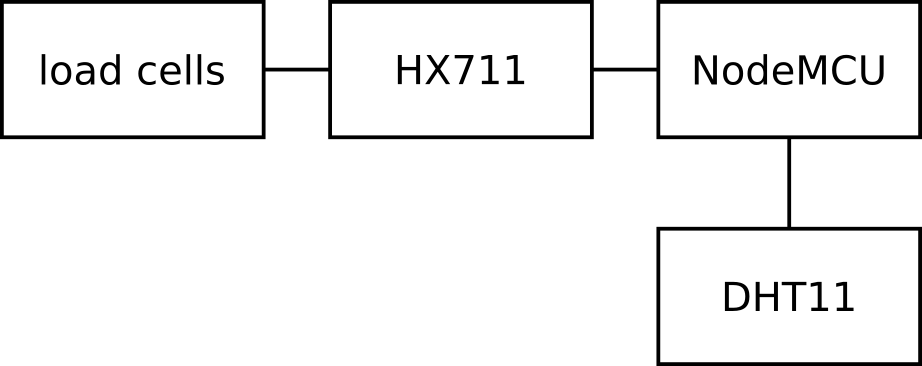
\includegraphics[width=0.7\textwidth]{latex/img/device_scheme.png}
  \caption{General scheme of the device.}\label{img:loadcells_scheme}
\end{figure}

\subsection{NodeMCU}
Programming the NodeMCU is as easy as writing Arduino code, provided that the support for Esp8266 is installed and the appropriate board is selected \footnote{\url{https://www.instructables.com/id/Quick-Start-to-Nodemcu-ESP8266-on-Arduino-IDE/}}.

\subsection{Weight - load cells + HX711}
A Wheatstone bridge configuration for four load cells is used \footnote{\url{https://www.aliexpress.com/item/1PCS-DIY-50Kg-Body-Load-Cell-Weighing-Sensor-Resistance-strain-Half-bridge/32597969753.html?spm=2114.13010608.0.0.pC56uP}} \footnote{\url{http://www.instructab
les.com/id/Make-your-weighing-scale-hack-using-arduino/, https://www.sparkfun.com/products/13878?_ga=1.186640489.1126097763.1485380550}}; see \autoref{img:loadcells_scheme}. Since the signal is too weak to be detected directly by the board, a HX711 amplifier is used; in the figure the schematics of connections to the board are shown.


In order to make the HX711 work, the library \texttt{HX711.h} is used \footnote{\url{https://github.com/bogde/HX711}}. The relevant code follows:
\begin{lstlisting}[language=C]
#include "HX711.h"
// set the pins used by the amplifier
#define HX711_SCK_PIN  D1         
#define HX711_DOUT_PIN D2
// create a HX711 object
HX711 scale;                      
scale.begin(HX711_DOUT_PIN,HX711_SCK_PIN);
scale.power_up(); // turn on the scale
scale.power_down(); // turn off the scale
// the value of myscale is obtained by calibrating 
//   the scale with known weights
scale.set_scale(myscale);         
// reset the scale to 0
scale.tare();                     
// get weight (tare and scale)
float weight = scale.get_units(); 
// get value of weight without tare 
float weight_raw = scale.read();
\end{lstlisting}

\label{topic:scale_tare}
Although, as shown in the code, it is possible to tare the scale with methods internal to the HX711 library, it is preferable to set up the tare with an external code: in order to reduce the calculations made on the NodeMCU and to make it more portable (i.e. requiring the least hands-on manteinance, allowing a remote intervention) such setup is done on Thingspeak: see \autoref{code:ts:tare}. \\
Apart of that, there are other advantages here. A big problem with the scale was its recalibration at each "reboot", so that the weight had to be removed and put on again; since the calibration is now done online, once set there is no need to remove weights at reboots. \\

A \textbf{known problem} whith this system: bumps (even small ones) could cause a rescaling of the non-calibrated readings, compromising the values. 

\begin{figure}[!htb] 
  \centering
  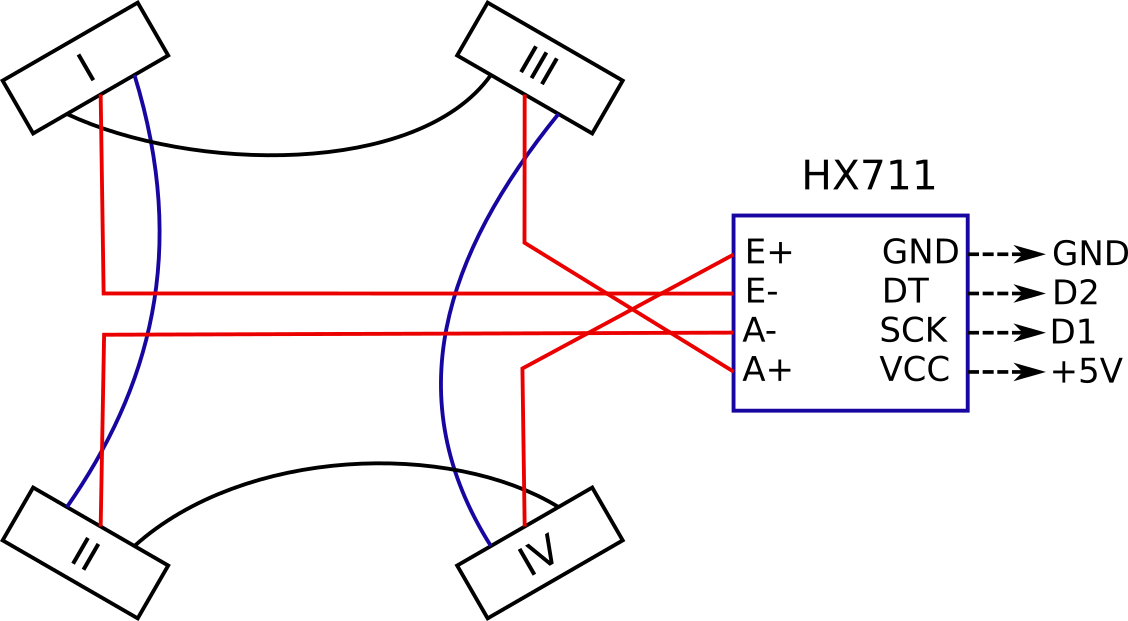
\includegraphics[width=0.65\textwidth]{latex/img/loadcells_scheme.png}
  \caption{The Wheatstone bridge configuration for load cells, connected to the HX711 amplifier; connections from HX711 to NodeMCU board.}\label{img:loadcells_scheme}
\end{figure}


\begin{figure}[!htb]
  \centering
  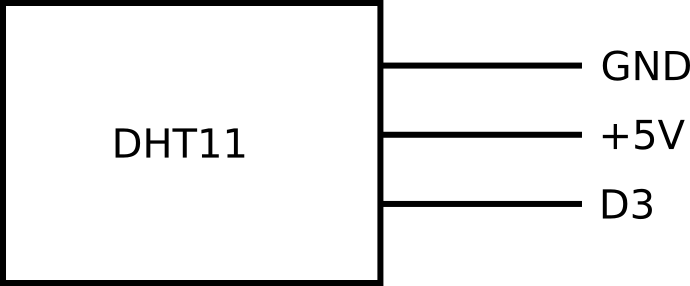
\includegraphics[width=0.4\textwidth]{latex/img/dht_scheme.png}\label{img:dht_scheme}
  \caption{The schematics of DHT11}
\end{figure}

\subsection{Temperature and humidity - DHT11}
A DHT11 sensor is used to get measures of temperature and humidity. The related schematics is in \autoref{img:dht_scheme}.

The library used is \texttt{DHT.h} and the relevant code is \footnote{\url{https://github.com/adafruit/DHT-sensor-library}, \textbf{needs} \url{https://github.com/adafruit/Adafruit_Sensor}}:

\begin{lstlisting}[language=C]
#include "DHT.h"
#define DHTTYPE DHT11
#define DHT11_PIN D3             // signal pin (has to be digital)
DHT dht(DHT11_PIN, DHTTYPE);     // create a DHT11 object
float t = dht.readTemperature(); // read values
float h = dht.readHumidity();
\end{lstlisting}








\include{latex/coding}
\section{Thingspeak.com}
As far as data visualization is concerned, the website Thingspeak.com, powered by Matlab plugins, has been the platform of choice. Provided that one has an account (a free plan exists), the website allows the creation of a \textit{channel}, which can contain up to 8 fields remotely updated with the provided API. \\

On NodeMCU boards, the following code starts a server connection

\begin{lstlisting}[language=C]
#include <ESP8266WiFi.h>
const char* server = "api.thingspeak.com";
String apiKey = "..........";     //  Enter the Write API key from ThingSpeak
WiFiClient client;
WiFi.begin(ssid, pass);
  while (WiFi.localIP().toString() == "0.0.0.0") 
  {
    delay(500);
    Serial.print(".");
  }
  Serial.println("WiFi connected");
\end{lstlisting}

while a String must be created to post it to the server:

\begin{lstlisting}[language=C]
if (client.connect(server, 80)) 
  {
    String postStr = apiKey;
    postStr += "&field1=";
    postStr += String(my_measure);
    postStr += "\r\n\r\n";
    client.print("POST /update HTTP/1.1\n");
    client.print("Host: api.thingspeak.com\n");
    client.print("Connection: close\n");
    client.print("X-THINGSPEAKAPIKEY: " + apiKey + "\n");
    client.print("Content-Type: application/x-www-form-urlencoded\n");
    client.print("Content-Length: ");
    client.print(postStr.length());
    client.print("\n\n");
    client.print(postStr);
  }
  client.stop();
\end{lstlisting}


\section{Data}
A very simple, yet satisfactory, approach has been taken to the elaboration of data: a sample over one or more days is considered, of which the weight-temperature points are fitted with a linear function. Assuming that the weight variation is neglectable with respect to the dependence on temperature of the response of the load cells, which is usually a decent assumption, the relation found corrects the instrumental noise:
\[ w_{\mathrm{vero}}[i] = w_{\mathrm{misurato}}[i] - (w_0 + m*T[i]) \]
It is worth noting that without correction the uncertainty is of order $0.01 kg$, so depending on the aim of the project may be that no correction is necessary to obtain an acceptable result.

The Matlab code, which can be directly used in a \textit{visualization} on Thingspeak.com, is presented:
\begin{lstlisting}[language=Matlab]
%%%%%%%%%%%%%%%%%%%%%%%
% this code gets data (weight, temperature) from Pesatura Arnie (ChID 350718)
% the correlation between the two variables is used to clean weight data
% so they are not subject to temperature variation
% the results are then averaged and displayed (original data vs. clean data) 

% read/write variables
writeChId = ......; % channel write id
writeKey = '.....'; % channel write API key
readChId = .......; % channel read id
readKey  = '.....'; % channel read API key

% retrieve last 100 data from Fields 1 and 2
npoints = 3*24*7;
[dataWeight,timestamps] = thingSpeakRead(readChId,'NumPoints',npoints,'Fields',1);%,'ReadKey',readKey);
dataTemperature = thingSpeakRead(readChId,'NumPoints',npoints,'Fields',2);%,'ReadKey',readKey);
dataHumidity = thingSpeakRead(readChId,'NumPoints',npoints,'Fields',3);
oldW = dataWeight; % keeps old measure
% clean data, using correlation with Temperature
m = 0.01; % correlation coefficient
n_back = 2; % NB the temperature affects weight with a DELAY!
T0 = 3 
for i=1:npoints
    if(i<(n_back+1))
            Delta2 = dataWeight(i)-dataWeight(1)-m*(dataTemperature(i)-T0);
    else
            Delta2 = dataWeight(i)-dataWeight(1)-m*(dataTemperature(i-n_back)-T0);
    end
    dataWeight(i) = Delta2;
end
% find mean values
nmean = 40;
mean = [0,0];
mean_dataWeight = [];
mean_oldW = [];
mean_timestamps = timestamps(1:npoints/nmean);
for i=1:npoints
    mean(1) = mean(1) + dataWeight(i);
    mean(2) = mean(2) + oldW(i);
      if isequal(mod(i,nmean),0)
          mean_dataWeight(i/nmean) =  mean(1)/nmean;
          mean_oldW(i/nmean) = mean(2)/nmean;
          mean_timestamps(i/nmean) = timestamps(i-nmean/2); % center of interval
          mean = [0,0];
      end       
end
numel(mean_dataWeight);
numel(mean_oldW);
numel(mean_timestamps);

%% Visualize Data %%
prevision = [];
for i=1:npoints
    prevision(i) = -dataWeight(1)+m*(dataTemperature(i)-T0);
end
A = horzcat(dataTemperature,transpose(prevision));
B = horzcat(transpose(mean_dataWeight),transpose(mean_oldW));
thingSpeakPlot(mean_timestamps,B,'XLabel','time','YLabel','weight(kg)','Title','weight with respect to original weight','Legend',{'corrected','measured'});
\end{lstlisting}


\section{Battery monitoring}
If the device is powered by a battery, a simple way to monitor its discharging is reading from pin A0 with the configuration shown in \autoref{img:battery_scheme.png}.

\begin{figure}[!htb] 
  \centering
  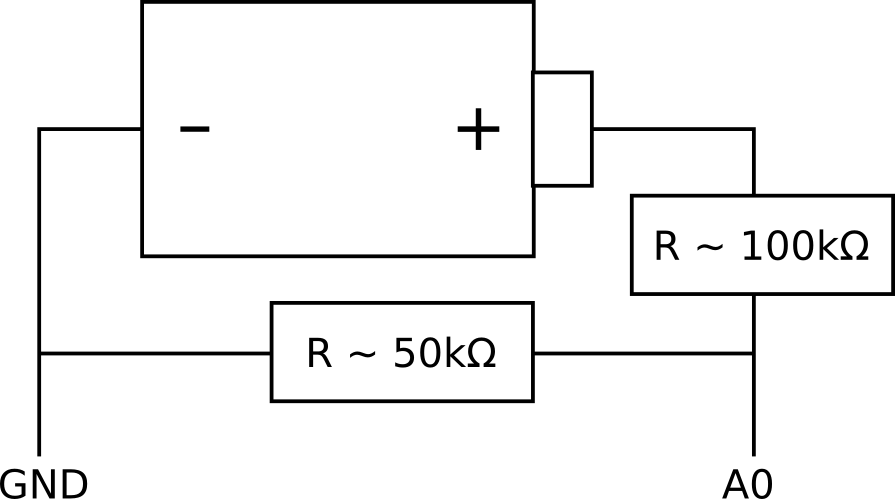
\includegraphics[width=0.65\textwidth]{latex/img/battery_scheme.png}
  \caption{The configuration needed to read battery level from pin A0.}\label{img:loadcells_scheme}
\end{figure}



\include{latex/rest}

\include{latex/codes}
%\lstinputlisting[language=C]{source.C}

%\printbibliography
\end{document}
